\documentclass[9pt,twocolumn,twoside]{../../styles/osajnl}
\usepackage{fancyvrb}
\journal{i524} 

\title{Twitter Heron}

\author[1]{Shahidhya Ramachandran}

\affil[1]{School of Informatics and Computing, Bloomington, IN 47408, U.S.A.}

\affil[*]{Corresponding authors: shahrama@iu.edu}

\dates{Technology paper 1, \today}

\ociscodes{Twitter Heron, Stream data, Real-time data Processing}

% replace this with your url in github/gitlab
\doi{\url{https://github.com/cloudmesh/sp17-i524/tree/master/paper1/S17-IR-2027}}


\begin{abstract}
Twitter Heron is a real-time analytics platform that was developed at Twitter for distributed streaming processing. The usage, architecture, features, performance and use cases of Twitter Heron are described in detail. Comparison of the capabilities of Twitter Heron and its predecessor Twitter Storm is summarized. A list of the other streaming technologies, which are used for streaming real-time data are discussed.\newline
\end{abstract}

\setboolean{displaycopyright}{true}

\begin{document}

\maketitle

\section{Introduction}

With the increase in the volume and diversity of data being generated in Twitter, the need to process these huge amounts of data in real-time along with an uprise in the number of use cases for real-time analytics, led to the necessity of having a real-time streaming system in place. This system should have the ability to process large amounts of data per minute; have sub-second latency and predictable behavior at scale; have high data accuracy in case of failure, ability to handle temporary traffic spikes and pipeline congestions; be easy to debug; and simple to deploy in a shared infrastructure as mentioned in \cite{TwitterHeron1}.

Twitter Heron is a real-time analytics platform that was developed at Twitter for distributed streaming processing \cite{www-openSourceHeron}. It was introduced at 'SIGMOD 2015' to overcome the shortcomings of Twitter Storm. Heron was open sourced under the Apache v2.0 license \cite{www-FlyFasterHeron}. Twitter initially introduced 'Storm' which served as the real-time data processing system and was later  replaced with 'Heron' that had enhanced capabilities and was architecturally more advanced than Storm \cite{www-FlyFasterHeron}. Since extension of Storm would require redesigning and switching to a new platform may lead to prolonged migration periods,Twitter decided to reuse existing components of Storm and made Heron fully backward compatible with Storm.  

\section{Architecture}
Heron's architecture is a process-based system instead of the thread-based system used in Storm. It is implemented using standard languages like Java, C++ and Python for efficiency, maintainability, and easier community adoption since it is open sourced. Heron allows for deployment in clusters by integrating with open source schedulers like Apache Mesos, Apache Aurora, Apache REEF, Slurm \cite{www-openSourceHeron}.

\subsection{Data Model}

The data model and API for Heron and Storm are same in order to maintain the backward compatibility. As explained in \cite{TwitterHeron2}, Heron contains topologies, each of which is a directed acyclic graph of spouts and bolts. Spouts generate the tuples that are given as input to the topology. Bolts are used for the computation. In the Heron topology, the number of tasks for every spout and bolt is specified. This decides the the degree of parallelism and grouping of the data as partitions when it moves through the spout and the bolt tasks. Heron’s tuple processing semantics are similar to that of Storm: At most once – A tuple is not processed more than once. Some tuples may not be processes even once by the topology; At least once – Every tuple is processed at least once. Some tuples may be processed more than once \cite{TwitterHeron2}.
\begin{figure}[htbp]
\begin{center}
\centering
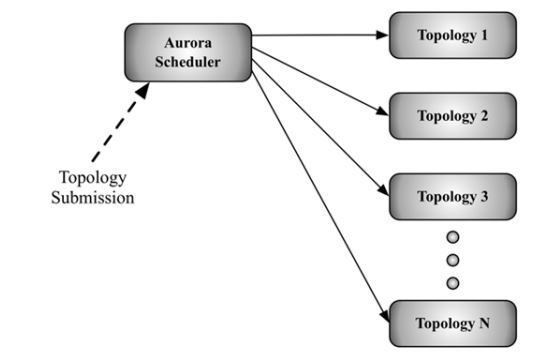
\includegraphics[width=\linewidth]{images/img1}
\caption{Heron Architecture \cite{TwitterHeron2}}
\label{fig:false-color}
\end{center}
\end{figure}
\subsection{Overview}
The architecture for Heron is shown in Figure 1. Heron API(spouts/bolts programming) is used to create and
deploy topologies to the Aurora scheduler through a command line specific to Heron. As shown in Figure 2, each topology consists of several containers, Topology Master is run by the first container,each of the other containers run Stream Manager, Metrics Manager and Heron Instances. Instances are the spouts/bolts in which the user code is run. Multiple containers can be launched on a single node. Based on the resource availability these containers are allocated and scheduled by Aurora. The metadata for the topology which includes user information(who ever launched the job), time of launch, and the execution details are kept in Zookeeper. Protocol buffers  are used for communication within the different processes.
\subsection{Topology Master}
As the name suggests the topology master is responsible for managing the entire topology and provides a consistent view of the topology throughout the process. A given topology can have only one TM and this is ensured by creating an ephemeral key in the Zoo keeper that can be easily identified by all processes run in that topology. 
\begin{figure}[htbp]
\begin{center}
\centering
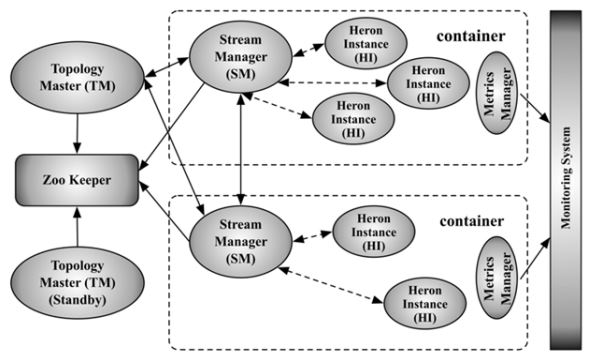
\includegraphics[width=\linewidth]{images/img2}
\caption{Heron Topology Architecture \cite{TwitterHeron2}}
\label{fig:false-color}
\end{center}
\end{figure}
\subsection{Stream Manager}
Stream Manager(SM) is used to route tuples that are sent and received by the Heron Instances. Heron uses a 'Backpressure' mechanism to control the flow of data into the system. If in a pipeline, all the stages do not process at the same rate then this may lead to tuples being dropped in order to clear the queued up buffers. This in turn will lead to loss of computational efficiency. Heron uses Spout Backpressure mechanism where the SM clamps the local spout to reduce the inflow of data. To maintain the processing rate across all SMs, the SM that is noticing slowed down performance sends a 'Start Backpressure' message to the other SMs. Once the other SMs receive this message they also clamp down their spouts until they get the 'Stop Backpressure' message from the SM that initialized the Backpressure \cite{TwitterHeron3}.
\subsection{Heron Instance}
Each Heron Instance(HI) executes a single task of the spout/bolt. Heron uses the two-threaded approach that employs a Gateway thread and a task execution thread as shown in the Figure 3. The Gateway thread is responsible for controlling all the communication and data movement in and out from the HI. It maintains TCP connections to the local SM and the metrics manager and receives the incoming tuples from the local SM. These tuples are sent to the Task Execution thread for processing. The task execution thread runs the user code. It evokes the 'execute' method in case of a bolt and the 'nextTuple' method in case of a spout.
\begin{figure}[htbp]
\begin{center}
\centering
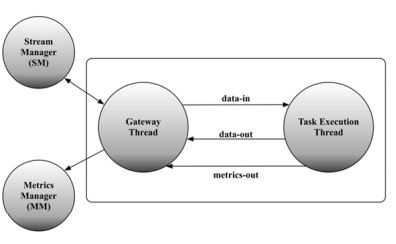
\includegraphics[width=\linewidth]{images/img3}
\caption{Heron Instance \cite{TwitterHeron4}}
\label{fig:false-color}
\end{center}
\end{figure}
\subsection{Metrics Manager}
The Metrics manager exports the system metrics and user metrics for the topologies. There is one metrics
manager for each container, to which the Stream Manager and Heron Instances report their metrics.
\subsection{Failure Handling}
When TM dies, the failed process is restarted in the container and the TM gets its state from the Zookeeper. The standby TM becomes the master and the master becomes the standby. When an SM fails, it rediscovers the TM to initiate a connection and get the physical plan to check if there are any changes in its state. When an HI dies, it is restarted within the container and contacts the local SM to get the physical plan \cite{TwitterHeron4}.

\section{Features}
\begin{itemize}
    \item API compatible with Storm: Back compatibility with Twitter Storm reduced migration time. 
    \item Task-Isolation: Every task runs in process-level isolation, making it easy to debug/profile
    \item Use of main stream languages: C++, Java, Python for efficiency, maintainability, and easier community adoption
    \item Support for backpressure: dynamically adjusts the rate of data flow in a topology during run-time, to ensure data accuracy
    \item Batching of tuples: Amortizing the cost of transferring tuples
    \item Efficiency: Reduce resource consumption by 2-5x and Heron latency is 5-15x lower than Storm’s latency \cite{www-FlyFasterHeron}
\end{itemize}
\section{Use cases}
Apart from being the primary streaming Engine of Twitter, Heron is being used for ETL, model enhancement, anomaly/fraud detection, IoT/IoE applications, embedded systems, VR/AR, advertisement bidding, financial, security, and social media\cite{www-openSourceHeron}. Microsoft deployed Heron on a YARN scheduler that was implemented with the Apache REEF framework \cite{www-HeronYARN}.

\section{Performance Comparison}
The performance of Heron was empirically compared with Storm using word count topology. This topology counts the distinct words in a stream generated from a set of 150,000 words. According to \cite{TwitterHeron5} all experiments were run on machines with dual Intel Xeon E5645@2.4GHZ CPUs, each consisting of 12 physical cores with hyper-threading enabled, 72GB of main memory, and 500GB of disk space. There are no out-of-memory (OOM) crashes (or any other failure due to resource starvation during scheduling), or long repetitive GC cycles. The Storm topologies were run in isolation, i.e. no process besides the kernel, Mesos slaves, and metric exporter daemons were run in the system. Heron was run in a shared cluster, with Linux “cgroups” isolation. As shown in Figure 4,though the topology throughput increases linearly for both Storm and Heron, the throughput is 10–14x higher for Heron than that of Storm. The end-to-end latency, shown in Figure 5, increases far more gradually for Heron than it does for Storm. Heron latency is 5-15x lower than Storm’s latency.Twitter reported in \cite{www-FlyFasterHeron} that with Heron, numerous topologies that aggregate data every second were able to achieve sub-second latencies and Heron was able to achieve the same with less resource consumption than Storm.
\begin{figure}[htbp]
\begin{center}
\centering
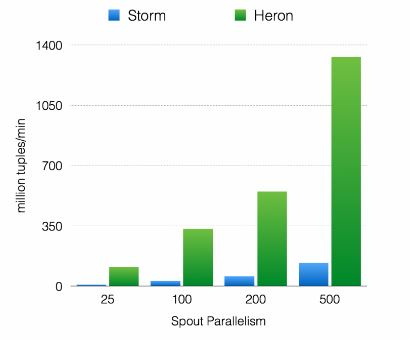
\includegraphics[width=\linewidth,height = 2.5in]{images/img4}
\caption{Throughput with acknowledgements enabled \cite{www-FlyFasterHeron}}
\label{fig:false-color}
\end{center}
\end{figure}
\begin{figure}[htbp]
\begin{center}
\centering
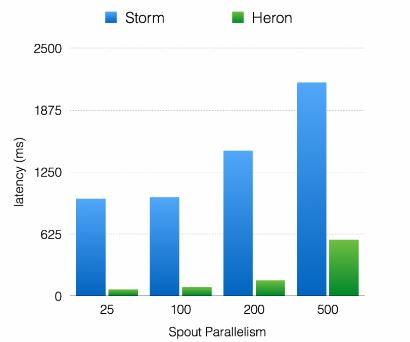
\includegraphics[width=\linewidth,height = 2.5in]{images/img5}
\caption{Latency with acknowledgements enabled \cite{www-FlyFasterHeron}}
\label{fig:false-color}
\end{center}
\end{figure}
\section{Other Streaming Engines}
\begin{itemize}
    \item Apache Flink: This streaming dataflow engine is programmed in Scala/Java/Python API. Flink offers batch processing, fault management, automated memory management, windowing features, etc \cite{www-StreamingTechs}.
    \item Apache Spark: It is a batch processing engine that emulates streaming via microbatching. It incorporates Scala, Java API, Python and R library \cite{www-StreamingTechs}.
    \item Apache Storm: It is is designed as a "topology" in the shape of a directed acyclic graph (DAG) with spouts and bolts acting as the graph vertices \cite{TwitterHeron6}.
    \item Apache Samza:Apache Samza uses Apache Kafka for messaging, and Apache Hadoop YARN to provide fault tolerance, processor isolation, security, and resource management \cite{www-ApacheSamza}.
    \item Apache Apex: Apache Apex is a YARN-native platform that unifies stream and batch processing. It is said to be scalable, performant, fault-tolerant, stateful, secure, distributed.
    \item Apache GearPump: It is an event/message based real time streaming engine. Per initial benchmarks we are able to process 18 million messages per second (message length is 100 bytes) with a 8ms latency on a 4-node cluster \cite{www-Gearpump}.
    \item Amazon Kinesis: It is a platform for streaming data on AWS, to load and analyze streaming data and to build custom streaming data applications for specific needs \cite{www-Kinesis}.
    \item Google MillWheel: Framework at google to implement stream applications. Users specify a directed computation graph and application code for individual nodes, and the system manages persistent state and the continuous flow of records \cite{GoogleMillwheel}.
    \item Apache Beam: A framework to create pipelines. The pipelines itself will executred on a streaming engine (such as Flink or Spark) \cite{www-StreamingTechs}.
\end{itemize}
\section{Conclusion}
Heron has been working effectively for large scale real-time data streaming at Twitter. The increase in throughput and reduction in latency of Heron has made it a useful tool for large scale processing. However it is essential to establish the required architecture to leverage the advantages of Heron. The effort and cost of setting up the Heron platform might be useful only for large scale systems. 

\bibliography{references}

\end{document}
